
\section{Method}
{Since concave factorization may not satisfy the IGM principle, we introduce an iterative action selection algorithm to ensure optimal joint action selection during training. It iteratively optimizes each agent's action selection with all other agent's actions and local utilities fixed. Due to the concave property of the mixing function, the iterative algorithm converges to global optimal actions. 
Note that this iterative action selection does not directly allow decentralized execution. To this end, we further leverage the soft actor-critic framework to train local factorized policies for distributed execution.
Figure \ref{framework} shows the architecture of our learning framework. There are four main
components in ConcaveQ : (1) a concave $Q_{tot}$ utilizing per-agent local utilities, where a concave function serves as the mixing network (2) an unrestricted joint action estimator $\hat{Q}^*$,
which serves as a baseline estimator of the true optimal value function $Q^*$ (3) an iterative action-selection module to seek the optimal joint action during training, and (4) a soft-policy network that allows for the utilization of a soft actor-critic network that consists of local policy networks and local value networks to perform decentralized execution. 




\subsection{Concave Mixing Network Design} 

The concave mixing network constrains the output of the network to be a concave function of the inputs, which covers a large class of functions and allows efficient inference via optimization over inputs to the network. Moreover, the concave feature ensures that maximizing the output of the network leads to only one solution. This means that theoretically there won't be local maximum or multiple solutions that may confuse the inference process. Concave mixing network has a suitable property specifically for value function factorization-based multi-agent reinforcement learning problems, that is, local maximization equals global maximization and it can be obtained through iterative methods, which is of great use in our case.


 We first consider a $k$-layer, fully connected network as shown in the left part of Figure \ref{framework}. A concave neural network is defined over the input $x$ for $i = 0, ...,k - 1$ using such architecture:
\setlength\intextsep{0pt}

\begin{equation}
\begin{array}{l}
\begin{aligned}
z_{i+1} = \left\{
\begin{aligned}
&W^{(z)}_0x + b_0, i = 0 \\
&r_i(W^{(z)}_i[z_1, ..., z_i]  + b_i), i = 1, ..., k - 2\\%, f(x;\theta) = z_k 
&-W^{(z)}_i[z_1, ..., z_i]  + b_i, i = k - 1
\end{aligned}
\right.  
\end{aligned}
\end{array}
\end{equation}

where $z_i$ denotes the layer activations, $r_i$ are non-linear activation functions, and $\theta = (W^{(z)}_{0:k-1}, b_{0:k-1})$ are the parameters of linear layers. We can model the concave mixing network as:
\begin{equation}
    f(x;\theta) = z_k
\end{equation}


{
\begin{theorem}
The mixing network $f$ is concave in $x$ provided that all $W^{(z)}_{1:k-1}$ are non-negative, and all functions $r_i$ are convex and non-decreasing.
\end{theorem}
}
 We delineate the proof and the detailed proof is provided in Appendices. The proof is simple and follows from the fact that non-negative sums of convex functions are also convex and that the composition of a convex and convex non-decreasing function is also convex, and that the negative of a convex function is a concave one \cite{convex_optimization}. In our framework, we satisfy the constraint that the $r_i$ should be convex non-decreasing via nonlinear activation units, specifically we adopt the rectified linear functions. The constraint that the $W^{(z)}$ terms be non-negative is somewhat restrictive, but because the bias terms can be negative, the network still has substantial representation power. In our multi-agent reinforcement learning setting, we model $Q_{tot}(s, \textbf{u}; \theta)$ using an input-concave mixing function and select actions under the concave optimization problem $u^*(s) = \text{argmax}_u{Q_{tot}(s, \textbf{u}; \theta)}$.  We have 4 layers, $k = 4$ and the weights  $W_{0:k-1}^{(z)}$ are generated by hypernetworks. Each hypernetwork takes the state
$s$ as input and consists of a single linear layer, succeeded by an absolute ReLU activation function, to generate the non-negative weights. 


\subsection{Iterative Action-Selection and Local Policies} We note that the optimal joint action of $Q_{tot}$ cannot be obtained directly from maximizing $Q_i$ since the mixing function is concave rather than monotonic. Hence it is almost impossible to directly find the maximum $Q_{tot}$ and the corresponding joint action selections $\textbf{u}^*$ such that $\textbf{u}^{*} = \text{argmax}_{\textbf{u}} \mathbb{E}[Q(s, \textbf{u})]$, as this takes $O(|U|^{|n|})$ iterations to find the maximum. One of the key insights underlying this method is that although it is impractical to find  ${\textbf{u}^*}$ directly: however, its local estimation and local optimum $\textbf{u}^* = \text{argmax}_\textbf{u}\mathbb{E}[Q^*(s, \tau, \cdot)]$, which takes $O(|U|*{|n|})$ time, is possible to find which will update the concave mixing network and local policy network asymptotically. 




To illustrate this problem, we consider the comparison between the action selection from the monotonic mixing network and concave mixing network: in value-based methods with a monotonic mixing network, each agent chooses $u^i_t = \text{argmax}(q^i(\tau^i_t))$, i.e. each agent chooses the action with the best local value thus getting an optimal global value; however, when the utilizing a concave mixing network for a more general value function factorization, we can maximize $\mathbb{E}[Q^*(s, \tau, \cdot)]$ via iterative action selection.


Next, since the mixing network is non-monotonic (concave), we can no longer follow the IGM principle to adopt actions that maximize individual values from the local value networks. Instead, we adopt a soft actor-critic policy network that uses factorized policies to enable distributed execution, such that each local agent can choose the best action according to its local policy network which will be corrected by the concave value networks during training while exploiting auxiliary information for learning.  Under a soft-actor-critic paradigm, each agent can choose $u^i_t = \text{argmax} (\pi^i(\tau^i_t))$ such that  $\mathbb{E}[Q^*(s, \tau, \textbf{u})] = \text{max}(\mathbb{E}[Q^*(s, \tau, \cdot)])$. This ensures that the concave mixing network could factorize concave value functions while each local agent could choose their best actions based on local policy in a decentralized manner during execution. Previous studies have demonstrated that Boltzmann exploration policy iteration can guarantee policy improvement and optimal convergence with infinite iterations and complete policy evaluation. With factorized policy, we have local policy trained with the following: 
\begin{small}
\begin{equation}
\begin{array}{l}
\begin{aligned}
\mathcal{L}_{\pi}(\theta) &=\mathbb{E}_{\mathcal{D}}\left[\boldsymbol\alpha \log \boldsymbol{\pi}\left(\boldsymbol{u}_{t} | \boldsymbol{\tau}_{t}\right)-Q^{\pi}_{tot}\left(\boldsymbol{s_{t}}, \boldsymbol{\tau_{t}}, \boldsymbol{u}_{t}\right)\right] \\
&= -q^{\pi}\left(\boldsymbol{s}_{t}, \mathbb{E}_{\pi^{i}}\left[\text{q}^{i}\left(\tau_{t}^{i}, u_{t}^{i}\right)-\alpha^{i} \log \pi^{i}\left(u_{t}^{i} | \tau_{t}^{i}\right)\right]\right)
\end{aligned}
\end{array}
\end{equation}
\end{small}
% $q^{Concave}$ is the concave mixing network, and
where $\text{q}^{\pi}$ is the local value network with $u_i \sim \pi_i(o_i)$, $\mathcal{D}$ is the replay buffer for sampling training data, and the parameter $\alpha$ from soft-actor-critic controls how much the agents prefer actions with higher expected rewards over actions with more explorations. We introduce the training of the local value network and other components in the following sections. The algorithm has a more vital exploration ability and a higher level of generalization. 




\begin{figure*}[ht!]%
    \centering
    \subfloat[Punishment $p=0.0$]{
        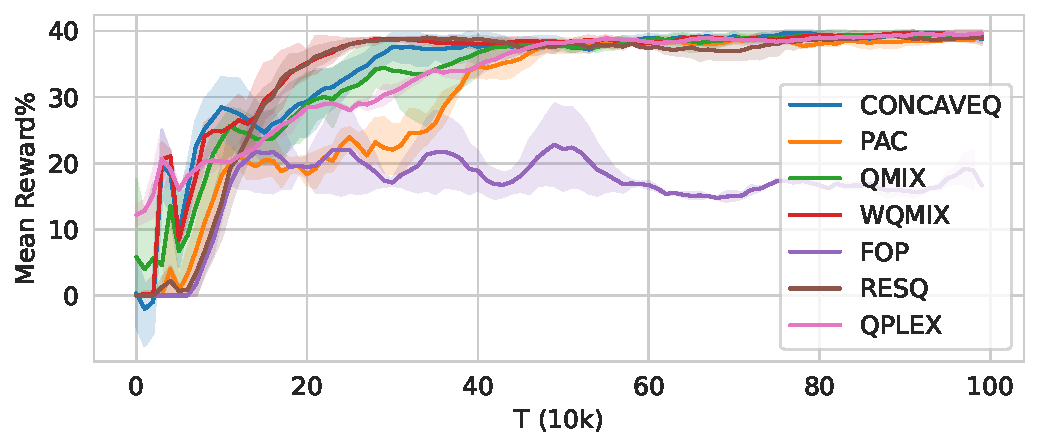
\includegraphics[width=0.5\linewidth]{new_figure/p_0_return_mean_comp_100_tab10.pdf}
        }%\hfill
    \subfloat[Punishment $p = -0.5$]{
        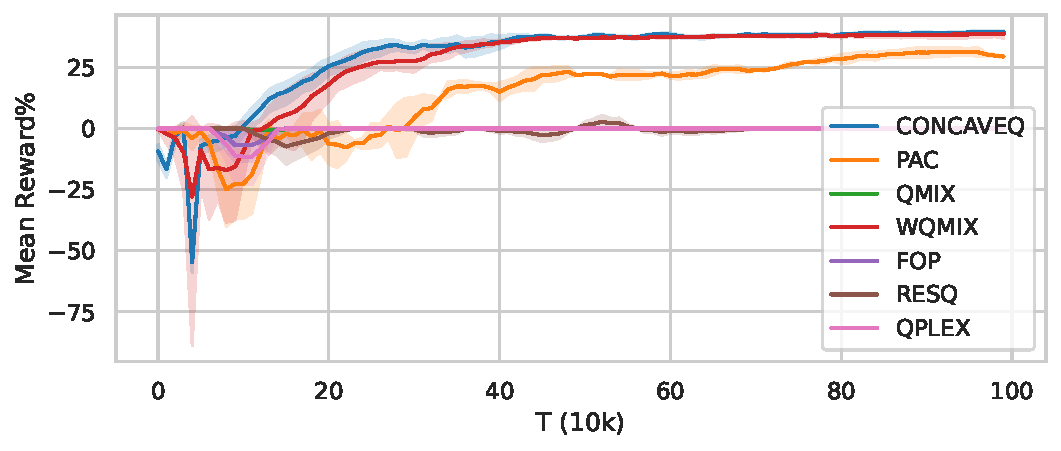
\includegraphics[width=0.5\linewidth]{new_figure/p_neg05_return_mean_comp_100_tab10.pdf}
        }\\
    \subfloat[Punishment $p = -1.5$]{
        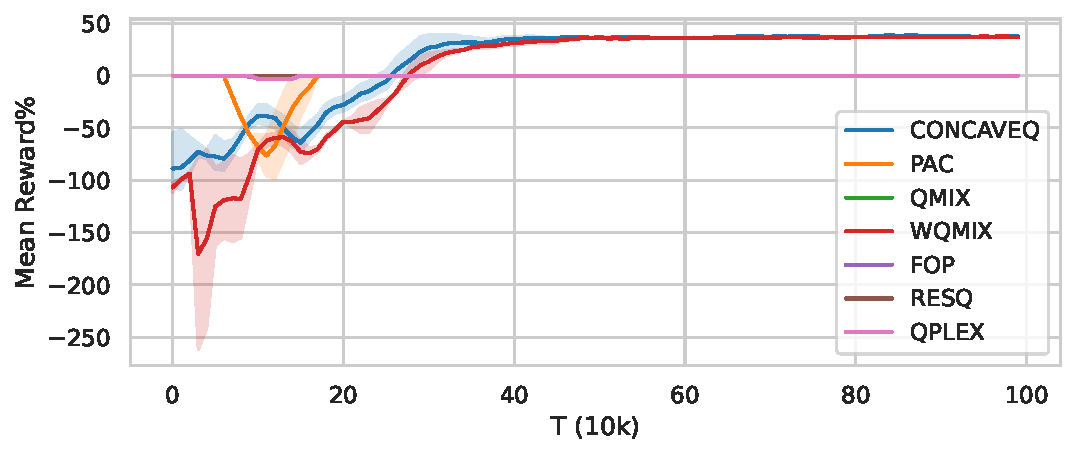
\includegraphics[width=0.5\linewidth]{new_figure/p_neg15_return_mean_comp_100_tab10.pdf}
        }%\hfill
    \subfloat[Punishment $p = -2.0$]{
        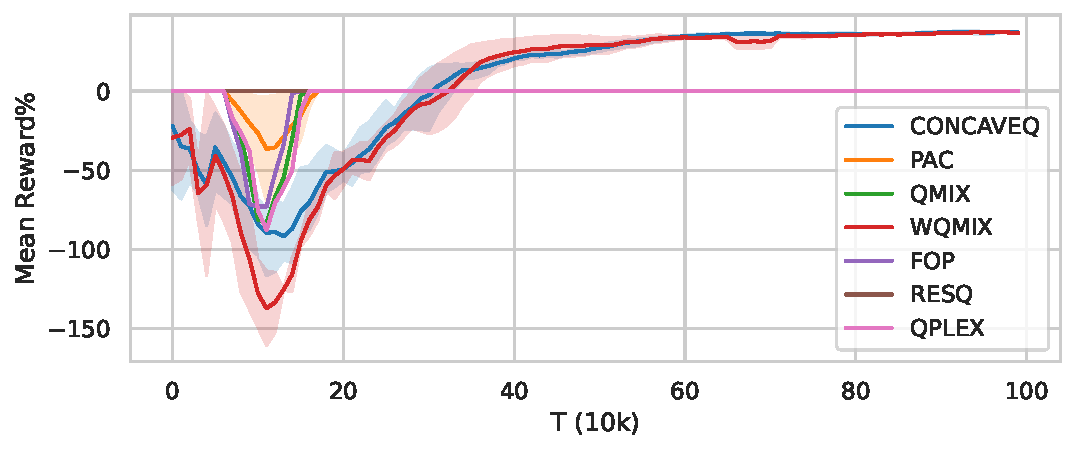
\includegraphics[width=0.5\linewidth]{new_figure/p_neg2_return_mean_comp_100_tab10.pdf}
        }\\    
    \caption{Average reward on the Predator-Prey tasks.}
    \label{exp_stag_hunt}
\end{figure*}

\subsection{Training ConcaveQ} 

We have presented the components of our approach so far. Next, we describe how to implement and train our novel RL algorithm that scales well under DEC-POMDP. During the decentralized execution phase, only the agent network (local policy in Fig.1) is active with actions chosen greedily from each local policy network as $u^i_t = \text{argmax} (\pi^i(\tau^i_t))$, ensuring full CTDE. 



The $\hat{Q}^*$ architecture (Green part in Fig. 1) is used as the estimator for ${Q}^*$ from unrestricted functions, where it serves as a mixing network using a feed-forward network that takes its local utilities. Together with the proposed concave mixing network, they are trained to reduce the following loss:

\begin{equation}
\mathcal{L}_{\hat{Q^{*}}}({\theta}) = \sum_{i}
(\hat{Q^{*}}(s, \boldsymbol{\tau}, \hat{\boldsymbol{u}}) - y_i)^2
\label{eq:qcentral_loss}
\end{equation}

\begin{equation}
\mathcal{L}_{{\text{ConcaveQ}}}({\theta}) = \sum_{i}
w(s,\textbf{u})(Q_{tot}(s, \boldsymbol{\tau},\textbf{u}) - y_{i})^2 
\end{equation}

% $\operatorname{argmax} Q_{tot}(\cdot, \mathbf{\tau})$ 
\noindent where $\hat{\boldsymbol{u}} = \operatorname{argmax}_{\boldsymbol{\hat{u}}} Q_{tot}(\boldsymbol{\tau^{\prime}}, \boldsymbol{\hat{u}^{\prime}}, s^{\prime}; \boldsymbol{\theta})$ is from local iterative action selection, $y_{i}=r+\gamma \hat{Q}^{*}(s', \boldsymbol{\tau^{\prime}}, \boldsymbol{\hat{u}})$ and 
$\boldsymbol{\theta^{\prime}}\ $ is the parameters of the target network that are periodically updated to stabilize the training.  $w(s,\boldsymbol{u})$ is the weighting function with $w = 1$ if $Q_{tot}(s, \tau, \boldsymbol{u}) - y_{i} < 0$,  $w = 0.5$ otherwise as suggested in WQMIX \cite{WQMIX}.  Then all components are trained in an end-to-end manner as:




\begin{equation}
\mathcal{L}(\theta) = \mathcal{L}_{\pi} +  \mathcal{L}_{\hat{Q^{*}}} + \mathcal{L}_{{\text{ConcaveQ}}}
\end{equation}


We provide detailed derivations and pseudo-codes for the training process in the appendices. 

